

\documentclass[a5paper,10pt, twoside]{article} % тип документа

\usepackage{hyperref}
\usepackage{fancyhdr}
\usepackage{import}
\usepackage{listings}

% Математика

\import{headers/}{math.tex}

%  Русский язык

\import{headers/}{russian.tex}

% Дефайны

\import{headers/}{my_defs.tex}

%\fancyhf{}
\renewcommand{\footrulewidth}{ .0em }
\fancyfoot[C]{\texttt{\textemdash~\thepage~\textemdash}}
\fancyhead[L]{Фракталы Ляпунова \hfil}
\fancyhead[R]{\hfil Лирисман Карина, Б01-001}

\pagestyle{fancy}

\graphicspath{{pics/}} % где лежат картинки

\counterwithin{figure}{section}

% Title Page
\title
{
\hfill \break	\hfill \break
\hfill \break	\hfill \break
Отчет по проекту

ФРАКТАЛЫ ЛЯПУНОВА
}
\author{Лирисман Карина, Б01-001}

%\setcounter{secnumdepth}{0}

\begin{document}

\maketitle


\thispagestyle{empty} % выключаем отображение номера для этой страницы

\newpage

\tableofcontents % Вывод содержания
\thispagestyle{plain}
\newpage


\section{Установка}

  \subsection{Библиотеки}
    \noindent Необходимо установить две библиотеки: \\
	  - Debian-based (Debian, Ubuntu, \ldots)
	  \begin{lstlisting}
	  	$ sudo apt-get install libsdl2-dev 
	  	$ sudo apt-get install libgtkmm-3.0-dev 
	  \end{lstlisting}
	  - RedHat-like (Fedora, CentOS, \ldots)
	  \begin{lstlisting}
	  	$ sudo yum install libsdl2-dev 
	  	$ sudo yum install libgtkmm-3.0-dev 
	  \end{lstlisting}

  \subsection{Скачивание}
    Перейти на GitHub и скачать папку \href{https://github.com/TheRedHotHabanero/AAL}{тут}, следуя указаниям в разделе $Code$.

  \subsection{Компиляция и запуск}
    \noindent Заходим в папку ляпунов
	  \begin{lstlisting}
	  	$ cd AAL/
	  \end{lstlisting}
	  Запустите команды для сборки:
	  \begin{lstlisting}
	  	$ mkdir build
	  	$ cd build
	  	$ cmake ..
	  	$ make
    \end{lstlisting}
	  Запустите команду для запуска исполняемого файла:
	  \begin{lstlisting}
	  	$ ./AAL
	  \end{lstlisting}

\section{Презентация программы}

  \subsection{Меню}

  При запуске программы отображается меню для выбора цветов, представляющих значения показателей Ляпунова
  желаемой точности, то есть количества итераций для вычисления показателя, и последовательности, которая будет использоваться.
  По нажатию "Подтвердить" запускается генерация и отображаются фракталы.
  Если пользователь не вводит последовательность при первом открытии меню, то последовательность генерируется случайным образом, 
  чтобы позволить пользователю открывать новые фракталы.
  Пользователь может получить случайную последовательность через консоль.
  Меню можно снова открыть, используя клавишу Esc для изменения цветов или изменения точности/последовательности.
  Если последовательность остается пустой при повторном открытии меню, то последняя последовательность будет учитываться 
  без необходимости повторного ввода пользователем последовательности.

  \subsection{Навигация}

  Навигация осуществляется стрелками направления (вверх, вниз, влево, вправо), что позволяет перемещаться на полэкрана.
  Масштабирование выполняется левым щелчком мыши, а область масштабирования обозначается белым квадратом вокруг указателя мыши.
  Уменьшение масштаба выполняется правой кнопкой мыши, чтобы вернуться к области перед масштабированием.
  Чтобы изменить степень масштабирования, используйте колесо мыши.

\section{Выполнение}
  
  \subsection{Управление SDL}

  Чтобы отобразить фрактал, использовалась SDL, которая представляет собой библиотеку, написанную на C, 
  и поэтому адаптировать ее к C++ с помощью оболочки, которой является класс WindowManager.
  Цель этого класса, таким образом, состоит в том, чтобы иметь возможность работать с SDL, избегая указателей, 
  и разрешить разделение между SDL и программой.
  Этот класс использует текстуру для изменения пикселей, которые нужно отобразить, и визуализацию 
  (которая является элементом SDL) для отображения текстуры на экране.
  Таким образом, можно легко отображать фрактал, не беспокоясь об операции на уровне SDL.
  Программа работает с циклом обработки событий, и для каждого интересующего нас события 
  можно обработать его с помощью функции обработки событий вне класса, работающего с SDL.

  \subsection{Генерация и отображение}

	Фракталы Ляпунова — это некоторое представление хаотической последовательности, вычисляемое из показателей Ляпунова.
	Алгоритм генерации двумерных фракталов Ляпунова на плоскости $[0,4] \times [0,4]$ делится на несколько этапов.
	Сначала выбираем последовательность A и B.
	Затем строится последовательность $S_n$ достаточно длинная, состоящая из повторения последовательности A и B, определенной ранее.
	Выбираем точку с координатами x, y в начальной плоскости.
	Затем определяем функцию $R_n = a$ если $ S_n = A $ и $R_n = b$ в противном случае.
	Затем строим последовательность $x_n$ считая $x_{{n+1}}=r_{n}x_{n}(1-x_{n})$ принимая за данность $x_0 = 0.5$.
	Затем вычисляем отмеченный показатель Ляпунова $\lambda$ при помощи формулы:
	\[\lambda = \lim_{N \to +\infty} \frac{1}{N} \sum_{n=1}^{N} \log | r_n(1-2x_n) |\]
	Затем для отображения фракталов на экране каждому показателю присваиваем цвет, чтобы иметь возможность 
  менять цвета на лету, которые представлены в RGB.

  \subsection{Оптимизация и многопоточность}

	Самой затратной операцией при вычислении показателя степени является логарифмирование, но так как вычисляются суммы логарифмов, 
  можно использовать свойство $\log(a) + \log(b) = \log(a \times b)$.
	Когда достигается определенный предел (здесь $1.10^{100}$: тип double позволяет достичь этих достаточно высоких значений), 
  логарифмируем произведение и прибавляем его к конечному результату.
  Таким образом, вычисляется меньше логарифмов и экономится время вычислений.
  Для повышения скорости расчета и отображения фракталов Ляпунова также используется распараллеливание.
  Получаем количество потоков процессора, а затем разрезаем генерацию из блока на 
  несколько блоков, каждый из которых соответствует области фрактала.
  Различные области фрактала отделены от количества «линий» на графике.
  Для этого используется нативную библиотеку <thread>, которую довольно легко использовать.
  Действительно, разделив вычисления показателей на разные потоки, можно сэкономить время при расчете фрактала.

  \subsection{Управление цветом}

	Цвета берутся из файла конфигурации.
  Затем сохраняются в таблице и распределяются по красной, зеленой и синей компонентам 
  разницу между максимальным и минимальным цветом по знаку экспоненты, затем цвет, которому эта разница приписана.
  Сохраняются максимальное и минимальное значения показателя степени вычисляемой области, чтобы создать шкалу цветов, 
  следующих за знаком. Для каждого компонента цвета цветовая разница умножается путем деления экспоненты на 
  соответствующую границу и, наконец, добавляется к сохраненному цвету.

	\subsection{Взаимодействие с пользователем}

  Для того, чтобы взаимодействовать с фракталом, нужно уметь преобразовывать экранные координаты в координаты Ляпунова.
  При этом используем область, которая определяет начальную и конечную координаты по обеим осям.
  Для преобразования делим для каждой координаты разницу между новой и старой точкой на ширину текстуры, 
  затем умножаем на текущую ширину и добавляем начало координат.

  \subsubsection{Увеличение, зум}

  При масштабировании извлекаем область путем преобразования координат экрана и вычисляем область 
  для отображения с этой областью.
  Чтобы иметь возможность уменьшать масштаб, сохраняем каждую область перед масштабированием, которую помещаем в стопку.
  С каждым щелчком правой кнопкой восстанавливаем эту область и пересчитываем, чтобы заново отобразить старый фрактал.

  \subsubsection{Перемещение}
  
  Зона, в которую мы хотим переместиться, рассчитывается по текущему региону путем добавления половины экрана.
  При попытке выйти за границу, регион прилипнет к границе.

  \subsection{Меню}
  Меню было сделано с помощью библиотеки <GTKmm>, C++ версии GTK+, в частности графической библиотеки GIMP.
  Она имеет множество классов, позволяющих пользователю очень легко создавать графические интерфейсы и навигационные меню.
  Поэтому была выбрана эту библиотеку для реализации меню: есть много виджетов, - селекторы цветов или даже области ввода 
  текста, позволяющие пользователю выбирать последовательность и цвета между другими.
  Меню в основном использует несколько небольших функций, которые упрощают заполнение файла конфигурации.
  Решено записать различные варианты выбора пользователя в файл конфигурации, чтобы иметь возможность легко 
  и быстро извлекать значения между различными классами, например, без необходимости использовать аксессор.
  Меню может записывать различные цвета в форме 255 255 255, введенную последовательность, а также точность, 
  желаемую пользователем в файле конфигурации.

\section{Выбор}

  \subsection{Язык}
  
  Решено использовать язык C++, потому что он быстрый, что важно для рассчетов фракталов, а также для 
  развития собственных навыков программирования.

  \subsection{Графическая библиотека}

	Использована SDL, потому что это неизвестная мне библиотека, таким образом освоен новый инструмент для работы.
  Дополнительно, другие библиотеки показались менее подходящими для попиксельного отображения.
  Еще использована GTKmm для создания меню из-за простоты использования для создания графического интерфейса.

\section{Аналитическая механика}

    \paragraph{Причастность к курсу МФТИ: }

    в первой половине учебного семестра активно изучались темы по теории устойчивости Ляпунова.
    Введены понятия фазового пространства, понятие о бифуркации. 

    \paragraph{Цель: }
    темы бифуркации прямо не были отражены в предложенных задачах, хотя показались мне 
    интересными и важными. Таким образом, для углубления своих знаний по курсу, было решено 
    самостоятельно изучить эту тему.
    
    \paragraph{Выбор задачи: }
    в Интернете я нашла статьи по фракталам Ляпунова, меня привлекли красивые картинки, и я 
    захотела посмотреть, какими они могут быть еще, и в итоге было решено написать программу 
    для фракталов Ляпунова.

\section{Скриншоты}

\newpage

  \begin{center}
    \begin{figure}[h!]
        \center{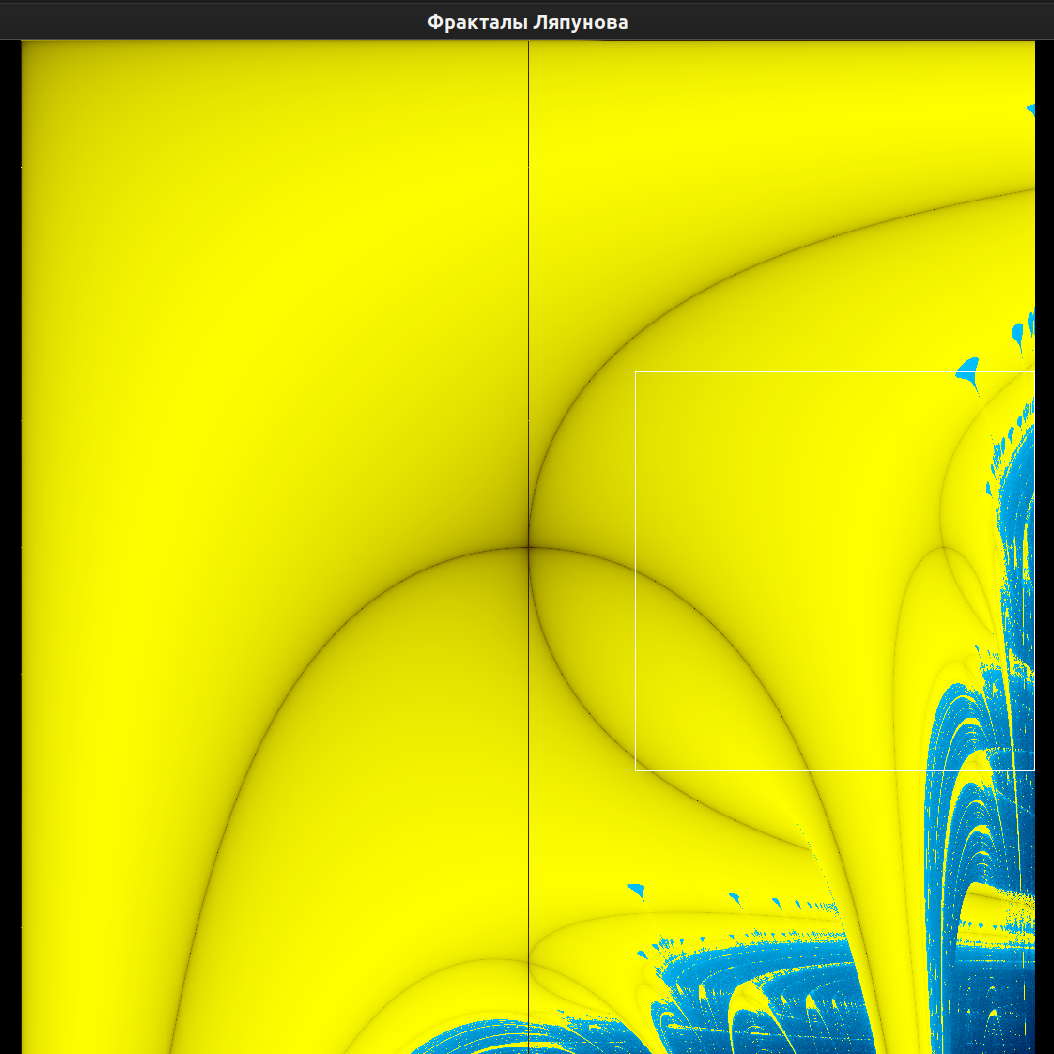
\includegraphics[width=0.5\linewidth]{pic1.png}}
        \caption{Последовательность AB}
    \end{figure}
  \end{center}

  \begin{center}
    \begin{figure}[h!]
        \center{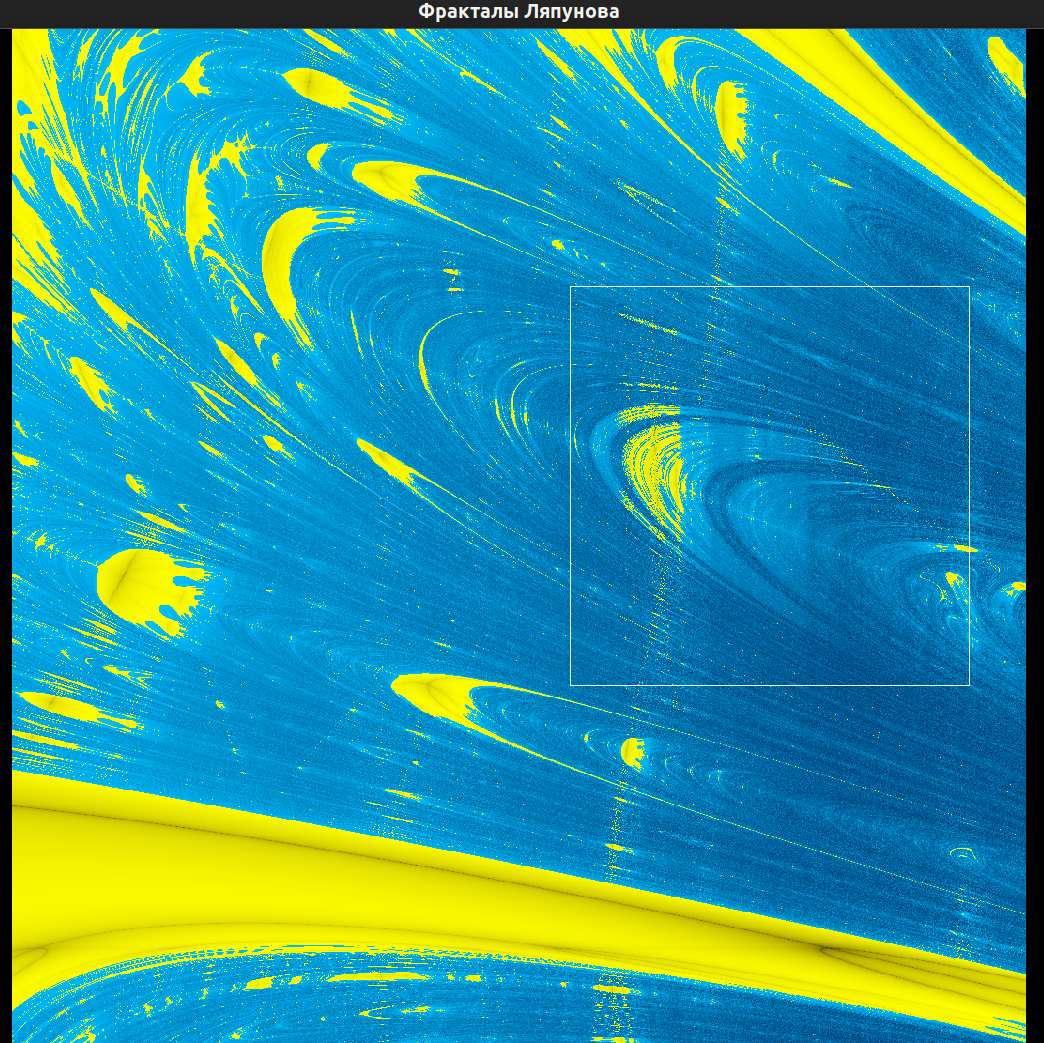
\includegraphics[width=0.5\linewidth]{pic5.png}}
        \caption{Последовательность BBBBBBBAAAAAAA}
    \end{figure}
  \end{center}

\newpage

  \begin{center}
    \begin{figure}[h!]
        \center{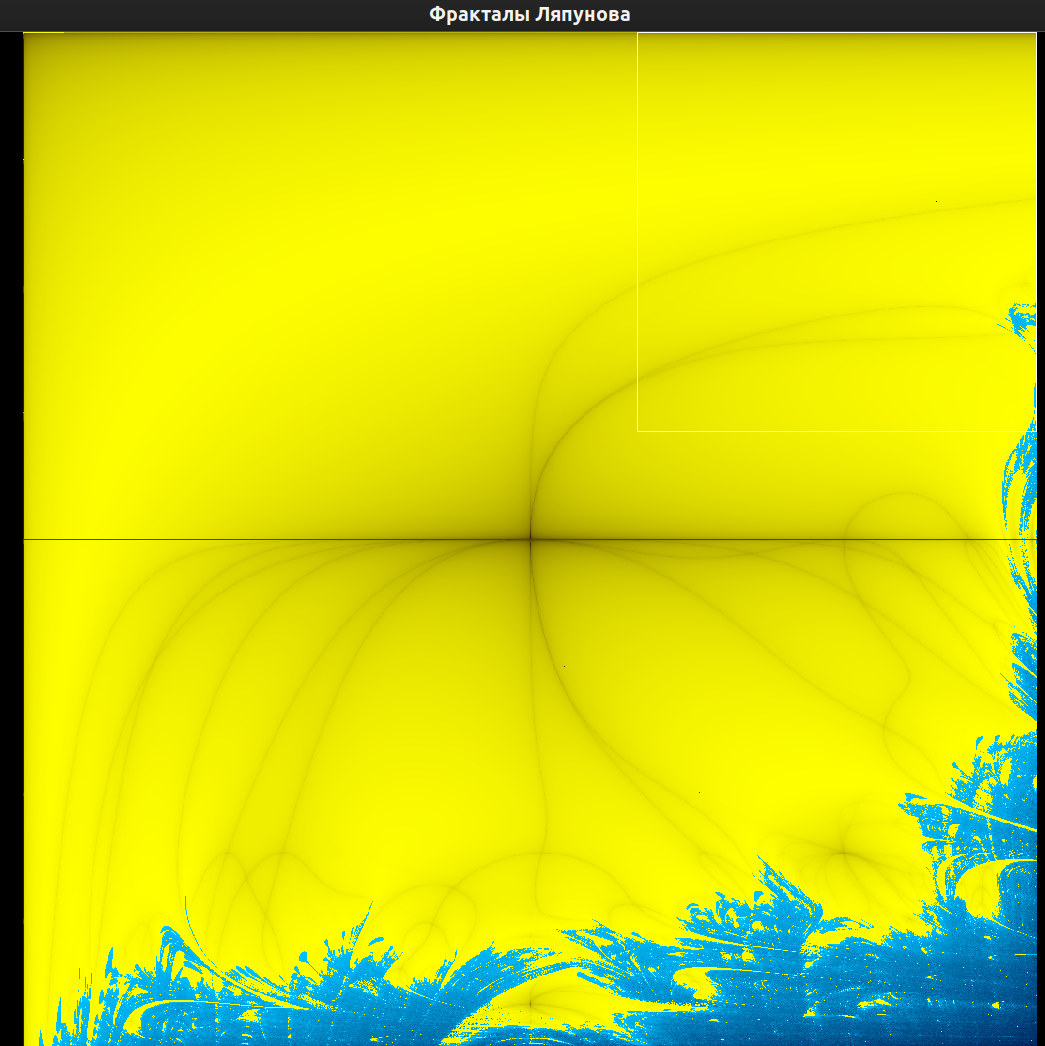
\includegraphics[width=0.5\linewidth]{pic3.png}}
        \caption{Последовательность BABBBAABB}
    \end{figure}
  \end{center}
  
    \begin{center}
    \begin{figure}[h!]
        \center{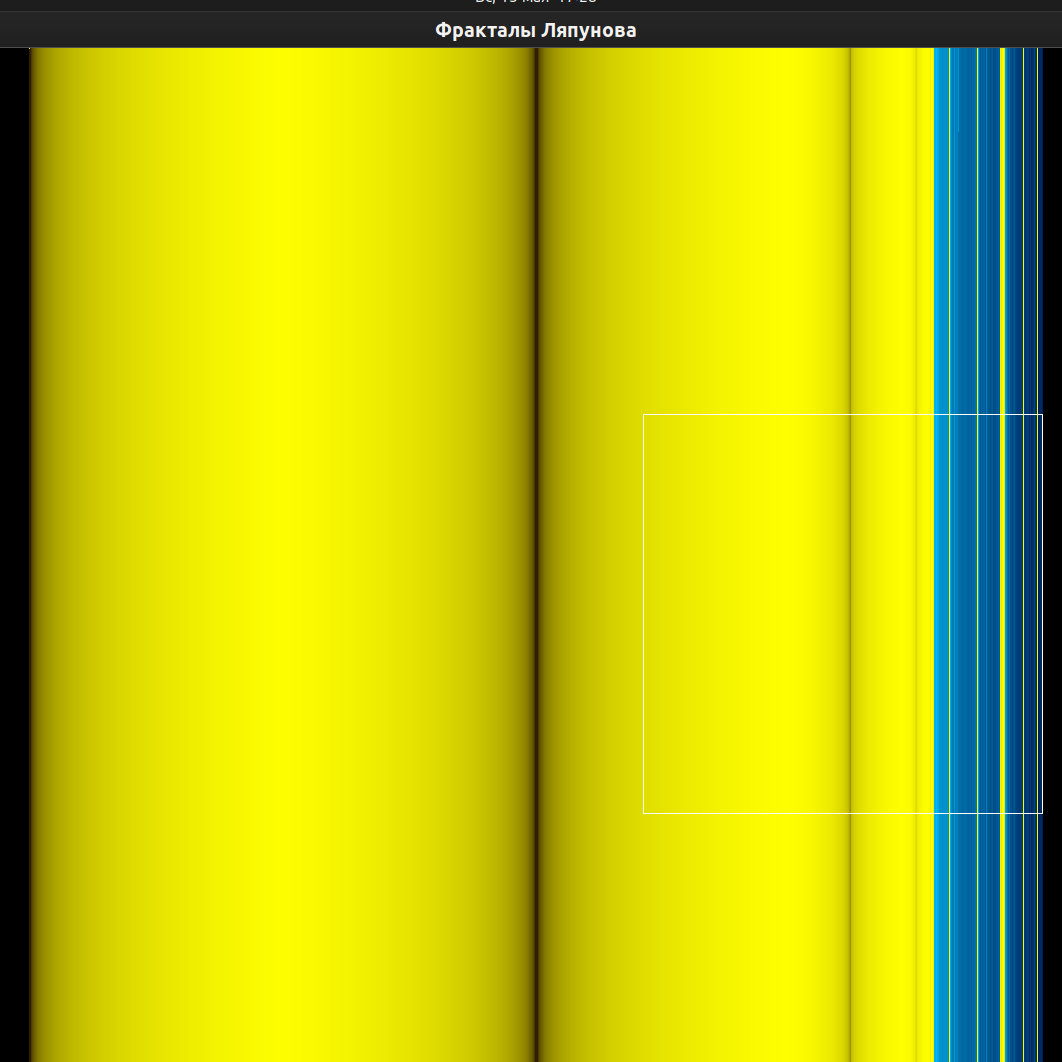
\includegraphics[width=0.5\linewidth]{pic4.png}}
        \caption{Последовательность AAAA}
    \end{figure}
  \end{center}


\end{document}